\section{Diversity in Critiques}
\label{sec:div}
\begin{figure}
\centering
\begin{minipage}{.45\textwidth}
  \centering
  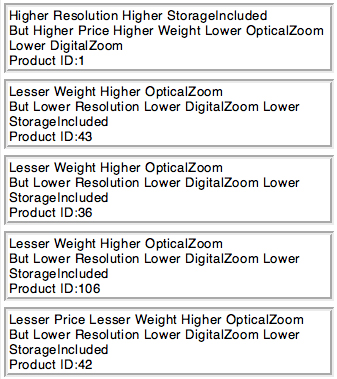
\includegraphics[width=1\linewidth]{figures-bharath/diversity1.jpg}
  \caption{Before diversifying critique strings}
  \label{fig:beforeDiv}
\end{minipage}%
\;\;\;\;\;\;
\begin{minipage}{.45\textwidth}
  \centering
  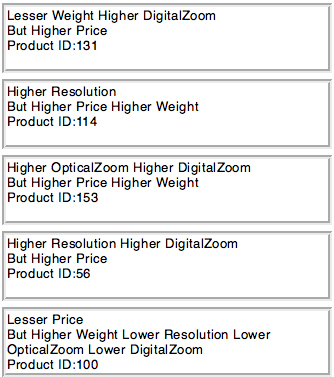
\includegraphics[width=1\linewidth]{figures-bharath/diversity2.jpg}
  \caption{After diversifying critique strings}
  \label{fig:afterDiv}
\end{minipage}
\end{figure}

In a live user-study conducted by \cite{aprioriUserStudy} to compare Apriori based critiquing with unit critiques, a number of trialists complained that their the compound critiques were often too similar to each other and hence they didn't have many options in each cycle.
As shown in Figure \ref{fig:beforeDiv} the same problem exists in MAUT based critiquing also.
In the first few cycles, an average user does not have a good understanding of the product space and also different trade-offs that exist between the product features.
Diverse critiques help educate a user about the product space relatively quickly and hence can lead to efficient recommendation sessions.
But in an attempt to make the critiques diverse, the recommender will have to choose a few sub-optimal products as the top $K$ products in every cycle.
So, there is a risk of having prolonged sessions because of this.

The default strategy for selecting the short-list of $K$ products is to select $K$ products that have highest utility.
Instead, we use a variant of \textit{\textbf{Bounded Greedy Selection}} algorithm described in \cite{boundedGreedy} to select the top $K$ products.
The main idea of this approach is that we select products with a high utility while minimizing the product's average similarity to the cases/compound critiques selected so far.
A metric that is similar to Equation \ref{eq:quality} is used to compute $Quality$ scores of products in each cycle.
\begin{equation}
\label{eq:quality}
Quality(c, P) = \alpha * utility(c) + (1-\alpha)*critiqueSim(c, P)
\end{equation}
%
The modified \textit{GenCritiqueItems(PM, IS)} function is given in Algorithm \ref{algo:div}.
\begin{algorithm}[ht]
  \SetKwInOut{Input}{input}\SetKwInOut{Output}{output}
  \DontPrintSemicolon
  %\Input{$PM$, $IS$}

  $R \gets \{\}$;\\
  $CB' \gets IS$;\\
  \For{ $i\gets0$ \KwTo $k$ }{
    Sort $CB'$ by $Quality(p, R, PM)$ for each case $p$ in IS; \\
    $R \gets R + First(CB')$;\\
    $CB' \gets CB' - First(CB')$;\\
  }
  \Return $R;$
  \caption{GenCritiqueItems(PM, IS)}
  \label{algo:div}
\end{algorithm}

\begin{algorithm}[ht]
  \SetKwInOut{Input}{input}\SetKwInOut{Output}{output}
  \DontPrintSemicolon
  %\Input{$i$, $R$, $PM$}

  $ret \gets \alpha \times utility(p, PM)$; \\
  \If {$R == \{\}$} {\Return $ret$;}
  \Else {
      $disSim \gets \frac{\sum_{r_j \in R} (1-critiqueSim(p,r_j))}{|R|}$;\\
      $ret += (1-\alpha) \times disSim$;\\
  }
  \Return $ret;$\\
  \caption{Quality(p, R, PM)}
  \label{algo:quality}
\end{algorithm}

\textit{critiqueSim(a, b)} returns the extent of overlap between the individual attribute directions of products $a$ and $b$.
We get the best results when $\alpha = 0.5$.
Introducing diverse critiques in every cycle results in significant improvement in the number of interaction cycles and it also improves user experience.
We will refer to Algorithm \ref{algo:quality} as DIV in subsequent sections.



